\date{}
\title{}
\date{}
\begin{document}
\begin{frame}
    \titlepage
\end{frame}

\makeatletter
\newenvironment<>{btHighlight}[1][]
{\begin{onlyenv}#2\begingroup\tikzset{bt@Highlight@par/.style={#1}}\begin{lrbox}{\@tempboxa}}
{\end{lrbox}\bt@HL@box[bt@Highlight@par]{\@tempboxa}\endgroup\end{onlyenv}}

\newcommand<>\btHL[1][]{%
  \only#2{\begin{btHighlight}[#1]\bgroup\aftergroup\bt@HL@endenv}%
}
\def\bt@HL@endenv{%
  \end{btHighlight}%   
  \egroup %
}
\tikzset{
    btHLbox/.style={
        fill=red!30,outer sep=0pt,inner xsep=1pt, inner ysep=0pt, rounded corners=3pt
    },
}
\newcommand{\bt@HL@box}[2][]{%
  \tikz[#1]{%
    \pgfpathrectangle{\pgfpoint{1pt}{0pt}}{\pgfpoint{\wd #2}{\ht #2}}%
    \pgfusepath{use as bounding box}%
    \node[text width={},draw=none,anchor=base west, btHLbox, minimum height=\ht\strutbox+1pt,#1]{\raisebox{1pt}{\strut}\strut\usebox{#2}};
  }%
}

\lst@CCPutMacro
    \lst@ProcessOther {"2A}{%
      \lst@ttfamily 
         {\raisebox{2pt}{*}}% used with ttfamily
         {\raisebox{2pt}{*}}}% used with other fonts
    \@empty\z@\@empty

\lstdefinelanguage
   [x8664gas]{Assembler}     % add a "x64" dialect of Assembler
   [x86masm]{Assembler} % based on the "x86masm" dialect
   % with these extra keywords:
   {morekeywords={CDQE,CQO,CMPSQ,CMPXCHG16B,JRCXZ,LODSQ,MOVSXD,%
                  POPFQ,PUSHFQ,SCASQ,STOSQ,IRETQ,RDTSCP,SWAPGS,.TEXT,.STRING,.ASCIZ,%
                  BEQ,LW,SW,LB,SB,ADDIU,J,BEQZ,BNEZ,BNE,%
                  MOVUPD,MULPD,MOVSD,MULSD,%
                  SHLADD,MOV,CMP.LT,TBIT.NZ,BR.RET.SPTK.MANY,%
                  ADDQ,POPQ,PUSHQ,RRMOVQ,MRMOVQ,RMMOVQ,IRMOVQ,%
                  <-,LL,SC,ADDI,ADDL,VMOVDQA,ADDQ,CMPL,JB,JBE,MOVL,CLTQ,
                  MOVW,PUSHW,MOV,ADD,SUB,INT,PUSH,MOV,ADD,REP,MOVSB,%
                  TESTQ,CMPQ,MOVL,MOVQ,ADDQ,JMPQ,XORQ,%
                  LEAQ,LEAL,LEA,RETQ,RET,POPL,POPW,PUSHL,PUSHW,%
                  LEAW,%
                  SUBQ,SYSCALL,.ASCII,CALLQ,MOVSLQ,JMP,ANDQ,SHRQ,MOVB,INCQ,TESTL,XORL,%
                  SHRL,LEAL,SARL,SUBL,IMULL,IMULQ,MOVDQU,PADDD,XORL,%
                  MOVZBL,MOVZB,SHRB,SRAL,SHRL,ANDL,%
                  CMOVNS,SRAL,SRAQ,MOVZBW,MOVZBQ,%
                  PADDW,PADDQ,MODUPS,MOVAPD,%
                  MOVL,RET,.GLOBL,%
                  },
    deletekeywords={eax,ebx,sp,si,cx,di,ds,cs,es,fs,dx,ax,bx,al,esi,ebp,ecx,rip,eip,edx,edi,rdi,esp},
    morecomment=[l]{\#},
    morecomment=[l]{\/\/},
    morecomment=[s]{/*}{*/},
    sensitive=false,
    keepspaces=true} % et

\lstalias[]{myasm}[x8664gas]{Assembler}

\lstdefinelanguage{JavaScript}{
  keywords={typeof, new, true, false, catch, function, return, null, catch, switch, var, if, in, while, do, else, case, break},
  ndkeywords={class, export, boolean, throw, implements, import, this},
  sensitive=false,
  comment=[l]{//},
  morecomment=[s]{/*}{*/},
  morestring=[b]',
  morestring=[b]"
}

\newcommand{\keywordstyle}{\sourcecodeprolight\bfseries\color{blue!30!black}}
\newcommand{\stringstyle}{\color{blue!20!black}\ttfamily}

\lstset{
    language=C,
    basicstyle=\sourcecodepro\EmptyMapping,
    escapechar=`,
    keywordstyle=\keywordstyle\EmptyMapping,
    identifierstyle=\sourcecodepro\EmptyMapping,
    numberstyle=\small\color{black!70},
    commentstyle=\color{red!60!black}\ttfamily\itshape,
    stringstyle=\color{blue!20!black}\ttfamily,
    ndkeywordstyle=\bfseries\color{blue!30!black},
    upquote=true,
}



\lstdefinestyle{medium}{
    basicstyle=\sourcecodepro\EmptyMapping\fontsize{12}{13}\selectfont,
    keywordstyle=\sourcecodepro\EmptyMapping\fontsize{12}{13}\selectfont\keywordstyle,
}

\lstdefinestyle{small}{
    basicstyle=\sourcecodepro\EmptyMapping\small,
    keywordstyle=\sourcecodepro\EmptyMapping\small\keywordstyle,
}

\lstdefinestyle{smaller}{
    basicstyle=\sourcecodepro\EmptyMapping\fontsize{11}{12}\selectfont,
    keywordstyle=\sourcecodepro\EmptyMapping\fontsize{11}{12}\selectfont\keywordstyle,
}


\lstdefinestyle{script}{
    basicstyle=\sourcecodepro\EmptyMapping\scriptsize,
    keywordstyle=\sourcecodepro\EmptyMapping\scriptsize\bfseries,
}



\newcommand{\z}[2]{\only<#1->{\myemph<#1|handout:0>{#2}}}
\newcommand{\zz}[3]{\only<#1-#2|handout:0>{\myemph<#1|handout:0>{#3}}}
\newcommand{\zzx}[3]{\only<#1-#2|handout:0>{#3}}
\newlength{\oneZero}
\settowidth{\oneZero}{\small\tt 0}
\newlength{\twoZeroes}
\settowidth{\twoZeroes}{\small\tt 00}

\usetikzlibrary{calc}

\begin{frame}{last time}
    \begin{itemize}
    \item C code and cache misses
    \item handling writes
        \begin{itemize}
        \item Q1: add to cache on write? (write-allocate)
        \item Q2: update next level immediately? (write-back)
        \end{itemize}
    \item dirty bits for write-back
    \end{itemize}
\end{frame}

\section{TLB}
\usetikzlibrary{arrows.meta, fit}
\begin{frame}<0>[label=twoLevelPtLookup]{two-level page table lookup}
\begin{tikzpicture}
\tikzset{
    >=Latex,
    pageNumber/.style={fill=blue!10,font=\fontsize{11}{12}\selectfont,inner sep=.5mm},
    pageNumberA/.style={fill=violet!30,font=\fontsize{11}{12}\selectfont,inner sep=.5mm,draw,thick,dotted},
    pageNumberB/.style={fill=brown!20,font=\fontsize{11}{12}\selectfont,inner sep=.5mm,draw,thick,dotted},
    pageOffset/.style={fill=green!20,font=\fontsize{11}{12}\selectfont,inner sep=.5mm},
    comp/.style={fill=yellow!10,font=\fontsize{11}{12}\selectfont,draw},
    memAccess/.style={alt=<all:7>{red, very thick}},
    pageNumberExpand/.style={alt=<all:11>{draw=red,very thick}},
    smallLabel/.style={fill=white,draw,thick,font=\fontsize{10}{11}\selectfont,inner sep=.5mm,align=center},
}
\node[pageNumberA] (addrLeftA) {11 0101 01};
\node[pageNumberB,anchor=west] (addrLeftB) at (addrLeftA.east) {00 1011 00};
\node[anchor=west,pageOffset] (addrRight) at (addrLeftB.east) {00 1101 1111};
\node[inner sep=0mm,draw=none,fit=(addrLeftA) (addrLeftB),alt=<1>{draw=red,very thick}] (addrLeft) {};
\begin{visibleenv}<all:1>
\node[below=1cm of addrLeft,xshift=2cm] (vpn split explain) {VPN --- split into two parts (one per level)};
\node[below=1cm of vpn split explain,font=\small] {
    this example: parts equal sized --- common, but not required
};
\end{visibleenv}
\begin{visibleenv}<all:2->
\node[draw,comp,below=1cm of addrLeftA,align=center,xshift=-1cm] (timesPte) {$\times$ \\ PTE \\ size};
\draw[->,thick] (addrLeftA) -- ++(0cm,-.5cm) -| (timesPte);
\node[font=\tt\fontsize{10}{11}\selectfont,draw,very thick,left=0.25cm of addrLeft,label={[align=center,font=\small]north:page table\\base register},yshift=-.5cm] (ptbr) {0x10000};
\node[draw,comp] (plus) at ([yshift=-1cm]timesPte.south) {+};
\draw[->,thick] (timesPte) -- (plus);
\draw[->,thick] (ptbr) |- (plus);
\end{visibleenv}

\begin{visibleenv}<all:3->
\node[below=1.5cm of plus,fill=violet!10,draw,very thick,minimum height=1cm,minimum width=15cm,xshift=5.5cm] (cache) {memory {\small (really cache)}};
\end{visibleenv}
\begin{visibleenv}<all:5->
\node[pageNumber] (addrLeftFinal) at ([xshift=9.6cm,yshift=-1cm]plus) {1101 0011 11};
\end{visibleenv}
\begin{visibleenv}<all:3->
\draw[->,thick,memAccess] (plus) -- (cache.north -| plus.south) node[midway,smallLabel] {1st PTE \\ addr.};
\node[above right=1cm and .5cm of plus,align=center,draw,comp,font=\small] (check) {valid, etc?};
\node[below=.75cm of check,draw,comp,align=center] (splitA) {split  \\ PTE parts};
\draw[->,thick] (cache.north -| splitA.south) -- (splitA.south);
\draw[->,thick] (splitA) -- (check);
\draw[->,thick] (check.north) -- ++(0,.75cm) node[above,font=\small,inner sep=.5mm] {cause fault?};
\end{visibleenv}

\begin{visibleenv}<all:4->
    \node[comp,align=center,right=.75cm of splitA,pageNumberExpand] (timesSize){$\times$ \\ page \\ size};
    \node[comp,align=center,right=1.25cm of timesSize] (plusB) {+};
    \draw[brown!60!black,->,thick,pageNumberExpand] (splitA) -- (timesSize);
    \draw[dotted,black,thick] ($(splitA.east)!0.5!(timesSize.west)$) -- ++ (0cm, .5cm) node[above,font=\fontsize{10}{11}\selectfont,align=center] {phys\\page \#};
    \draw[brown!60!black,->,thick,pageNumberExpand] (timesSize) -- (plusB);
    \draw[dotted,black,thick] ($(plusB.east)!0.5!(timesSize.west)$) -- ++ (0cm, .5cm) node[above,font=\fontsize{10}{11}\selectfont,align=center] {phys\\addr};
    \draw[memAccess,->,thick] (plusB) -- (plusB |- cache.north) node[midway,smallLabel]{2nd PTE \\ addr.};
    \node[comp,align=center,above=.5cm of plusB] (timesPteB) {$\times$ \\ PTE \\ size};
    \draw[brown!60!black,->,thick] (addrLeftB) -- ++(0cm,-.5cm) -| (timesPteB.north);
    \draw[brown!60!black,->,thick] (timesPteB) -- (plusB);
\end{visibleenv}

\begin{visibleenv}<all:5->
\node[right=.5cm of plusB,draw,comp,align=center] (splitB) {split  \\ PTE parts};
\draw[->,thick] (cache.north -| splitB.south) -- (splitB.south);
\node[above=.75cm of splitB,align=center,draw,comp,font=\small] (checkB) {valid, etc?};
\draw[->,thick] (splitB) -- (checkB);
\draw[->,thick] (checkB.north) -- ++(0cm, .75cm) node[above,font=\small,inner sep=.5mm] {cause fault?};
\draw[blue!50!black,->,thick] (splitB) -| (addrLeftFinal);
\end{visibleenv}

\begin{visibleenv}<all:6->
\node[anchor=west,pageOffset] (addrRightFinal) at (addrLeftFinal.east) {00 1101 1111};
%\draw[very thick,green!50!black,densely dotted] (addrRight) |- ([xshift=-.5mm,yshift=.5cm]splitA.north);
\draw[very thick,green!50!black,densely dotted,->] (addrRight) -| (addrRightFinal.north);
\end{visibleenv}
\begin{visibleenv}<all:3->
\node[inner sep=0mm,draw,label={[font=\fontsize{12}{13}\selectfont]south:physical address},fit=(addrLeftFinal) (addrRightFinal)] (addrFinal) {};
\end{visibleenv}

\node[inner sep=0mm,draw,label={[font=\fontsize{12}{13}\selectfont]north:virtual address},fit=(addrLeft) (addrRight)] (addr) {};
\begin{visibleenv}<all:5->
    \draw[->,thick,memAccess] (addrFinal) -- (cache.north -| addrFinal.south);
\end{visibleenv}

\begin{pgfonlayer}{bg}
\begin{visibleenv}<all:8,10>
    \node [fill=violet!5,fit=(timesPte) (splitA),draw,line width=0.125mm,dashed] (firstBox) {};
\end{visibleenv}
\begin{visibleenv}<all:9,10>
    \node [fill=brown!5,fit=(timesPteB) (splitB),draw,line width=0.125mm,dashed] (secondBox) {};
\end{visibleenv}

\begin{visibleenv}<all:12>
    \node [fill=black!5,fit=(timesPte) (splitA) (timesPteB) (splitB),draw,line width=0.5mm,dashed,label={south:MMU}] (mmu) {};
\end{visibleenv}
\end{pgfonlayer}
 
\begin{visibleenv}<all:8> 
\node [fill=white,fill opacity=0.9,anchor=north] at (firstBox.south) {first-level page table lookup};
\end{visibleenv}

\begin{visibleenv}<all:9> 
\node [fill=white,fill opacity=0.9,anchor=north] at (secondBox.south) {second-level page table lookup};
\end{visibleenv}
 
\begin{visibleenv}<all:10> 
\node [fill=white,fill opacity=0.9,anchor=north] at (firstBox.south) {first-level};
\end{visibleenv}

\begin{visibleenv}<all:10> 
\node [fill=white,fill opacity=0.9,anchor=north] at (secondBox.south) {second-level};
\end{visibleenv}

\begin{visibleenv}<all:11>
\node[fill=white,fill opacity=0.9,anchor=south,align=center] at (timesSize.north) {
    have physical page number \\
    need address of first byte of page 
};
\end{visibleenv}
\end{tikzpicture}
\end{frame}

\subsection{review: page table lookup (1)}
\usetikzlibrary{arrows.meta}
\begin{frame}{another view}
\begin{tikzpicture}
    \tikzset{
        addrPart/.style={draw,minimum height=.6cm},
        pt/.style={draw,ultra thick,minimum height=4cm,minimum width=3.25cm,align=center},
        pte/.style={draw,thin,minimum height=.6cm,minimum width=3.25cm,font=\small,fill=black!5},
        >=Latex,
        compute/.style={thick,->},
        computeB/.style={thick,->,dashed},
    }
    \node[addrPart,minimum width=4.25cm] (vpn1) {VPN part 1};
    \node[addrPart,right=0cm of vpn1,minimum width=4.25cm] (vpn2) {VPN part 2};
    \node[addrPart,right=0cm of vpn2,minimum width=5cm] (po) {page offset};

    \node[pt,below=1cm of vpn1,xshift=1cm] (first) {
        first-level \\
        page table \\
        ~ \\
        ~ \\
    };
    
    \node[draw,below=1cm of first,xshift=-.5cm] (ptbr) {page table base register};
    \draw[compute] (ptbr.east) -- ++(.5cm,0cm) |- ([xshift=-.5cm,yshift=-.5cm]first.south west) |- (first.south west);
    \node[pte] (pte1) at ([yshift=1.3cm]first.south) {page table entry};
    \draw[computeB] ([xshift=1.2cm]vpn1.south west) |- (pte1.south west);

    \node[pt,below=1cm of vpn2,xshift=1cm] (second) {
        ~ \\
        ~ \\
        second-level \\
        page table
    };
    
    \draw[compute] (pte1.east) -- ++(.25cm,0cm) |- (second.south west);
    
    \node[pte] (pte2) at ([yshift=2.8cm]second.south) {page table entry};
    \draw[computeB] ([xshift=1.2cm]vpn2.south west) |- (pte2.south west);
    
    \node[pt,below=1cm of po,xshift=1cm] (final) {
        physical page
    };
    \draw[compute] (pte2.east) -- ++(.25cm,0cm) |- (final.south west);
    \draw[computeB] ([xshift=1.2cm]po.south west) |- ([yshift=2cm]final.south west);
\end{tikzpicture}
\end{frame}


\subsection{review: page table lookup (2)}
\againframe<7>{twoLevelPtLookup}

\subsection{why cache page table entries?}
\usetikzlibrary{calc,positioning,patterns,shapes.callouts}

\begin{frame}{cache accesses and multi-level PTs}
    \begin{itemize}
    \item four-level page tables --- five cache accesses per program memory access
    \item L1 cache hits --- typically a couple cycles each?
    \item so add 8 cycles to each program memory access?
    \vspace{.5cm}
    \item not acceptable
    \end{itemize}
\end{frame}

\begin{frame}{program memory active sets}
\begin{tikzpicture}
\tikzset{
    mylabel/.style={font=\ttfamily},
    mybox/.style={draw,rectangle,minimum width=5cm,fill=white},
    myhigh/.style={draw,rectangle,line width=1mm, draw=blue!80!black,opacity=.3},
}
\node[mybox,minimum height=1cm,pattern=north west lines,pattern color=black!5!white] (kernel) {Used by OS};
\begin{pgfonlayer}{bg}
\node[right=1mm of kernel.north east,mylabel] (topLabel) {0xFFFF FFFF FFFF FFFF};
\node[right=1mm of kernel.south east,mylabel] {0xFFFF 8000 0000 0000};
\end{pgfonlayer}
\node[mybox, minimum height=.5cm, below=1cm of kernel] (stack) {Stack};
\begin{pgfonlayer}{bg}
\node[right=1mm of stack.north east,mylabel] {0x7F\ldots{}};
\end{pgfonlayer}
\node[mybox, minimum height=.5cm, below=1cm of stack] (heap) {Heap / other dynamic};
\node[mybox, minimum height=.5cm, below=0mm of heap] (data) {Writable data};
\node[mybox, minimum height=.5cm, below=0mm of data] (sdata) {Code + Constants};
\begin{pgfonlayer}{bg}
\node[right=1mm of sdata.south east,mylabel] (bottomLabel) {0x0000 0000 0040 0000};
\end{pgfonlayer}
\coordinate (memBottom) at ($(sdata.south east) + (0mm, -2mm)$);
\begin{pgfonlayer}{bg}
\draw[pattern=north west lines, pattern color=black!40!white] (kernel.north west) rectangle (memBottom);
\end{pgfonlayer}
\draw[fill=red] ([yshift=.1cm]stack.north west) rectangle ([yshift=-.15cm]stack.north east);
\draw[fill=red] ([yshift=.1cm]sdata.north west) rectangle ([yshift=-.15cm]sdata.north east);
\draw[fill=red] ([yshift=.1cm]heap.north west) rectangle ([yshift=-.15cm]heap.north east);

\node[right=.5cm of stack,align=left,yshift=-1cm] {
    small areas of memory active at a time \\
    one or two pages in each area?
};
\end{tikzpicture}
\end{frame}

% FIXME: hilight program memory layout picture?
\begin{frame}{page table entries and locality}
    \begin{itemize}
    \item page table entries have \myemph{excellent temporal locality}
    \item typically one or two pages of the stack active
    \item typically one or two pages of code active
    \item typically one or two pages of heap/globals active
    \vspace{.5cm}
    \item each page contains \myemph{whole functions}, arrays, stack frames, etc.
    \vspace{.5cm}
    \item<2-> needed page table entries are \myemph{very small}
    \end{itemize}
\end{frame}

\begin{frame}{page table entry cache}
    \begin{itemize}
    \item caled a \textbf{TLB} (translation lookaside buffer)
    \item \myemph{(usually very small) cache of page table entries}
    \vspace{.5cm}
    \item
    \begin{tabular}{l|l}
    L1 cache & TLB \\ \hline
        physical addresses & \myemph<2-3>{virtual\tikzmark{vpns} page numbers} \\
        bytes from memory & \myemph<2-3>{page table\tikzmark{copyPTE} entries} \\
        tens of bytes per block & \myemph<4-5>{one page table\tikzmark{onePerBlock} entry per block} \\
    usually thousands of blocks & \myemph<6>{usually tens of entries}\tikzmark{entries} \\
    \end{tabular}
    \end{itemize}
\begin{tikzpicture}[overlay,remember picture]
\begin{visibleenv}<2>
\node[my callout=copyPTE,align=left] at ([xshift=-6cm,yshift=-1cm]pic cs:copyPTE) {
    only caches the page table lookup itself \\
    (generally) just entries from the last-level page tables
};
\end{visibleenv}
\begin{visibleenv}<3>
\node[my callout=copyPTE,align=left] at ([xshift=-6cm,yshift=-1cm]pic cs:copyPTE) {
    virtual page number divided into \\
    index + tag
};
\end{visibleenv}
\begin{visibleenv}<4>
\node[my callout=onePerBlock,align=left] at ([xshift=-9cm,yshift=-1cm]pic cs:onePerBlock) {
    not much spatial locality between page table entries \\
    (they're used for kilobytes of data already)
};
\end{visibleenv}
\begin{visibleenv}<5>
\node[my callout=onePerBlock,align=left] at ([xshift=-9cm,yshift=-1cm]pic cs:onePerBlock) {
    {\tt 0} block offset bits
};
\end{visibleenv}
\begin{visibleenv}<6>
\node[my callout=entries,align=left] at ([xshift=-6cm,yshift=-.5cm]pic cs:entries) {
    few active page table entries at a time \\
    enables highly associative cache designs
};
\end{visibleenv}
\end{tikzpicture}
\end{frame}


\subsection{how TLB fits in page table lookup}
\begin{frame}{TLB and multi-level page tables}
    \begin{itemize}
    \item TLB caches \myemph{valid last-level page table entries}
    \item doesn't matter which last-level page table
        \vspace{.5cm}
    \item means TLB output can be used directly to form address
    \end{itemize}
\end{frame}

\usetikzlibrary{arrows.meta,fit,positioning,calc}

\begin{frame}<1-2>{TLB and two-level lookup}
\begin{tikzpicture}
\tikzset{
    >=Latex,
    pageNumber/.style={fill=blue!10,font=\fontsize{11}{12}\selectfont,inner sep=.5mm},
    pageNumberA/.style={fill=violet!20,font=\fontsize{11}{12}\selectfont,inner sep=.5mm},
    pageNumberB/.style={fill=brown!20,font=\fontsize{11}{12}\selectfont,inner sep=.5mm},
    pageOffset/.style={fill=green!20,font=\fontsize{11}{12}\selectfont,inner sep=.5mm},
    comp/.style={fill=yellow!10,font=\fontsize{11}{12}\selectfont,draw},
    memAccess/.style={alt=<all:0>{red, very thick}},
    pageNumberExpand/.style={alt=<all:0>{draw=red,very thick}},
    smallLabel/.style={fill=white,draw,thick,font=\fontsize{9}{10}\selectfont,inner sep=.5mm,align=center},
    ifMiss/.style={draw=blue!50!black,alt={<1>{dashed,opacity=0.25}}},
    ifHit/.style={draw=violet!50!black,alt={<2>{dashed,opacity=0.25}}},
    ifHitNoSkip/.style={draw=violet!50!black},
}
\node[pageNumberA] (addrLeftA) {11 0101 01};
\node[pageNumberB,anchor=west] (addrLeftB) at (addrLeftA.east) {00 1011 00};
\node[anchor=west,pageOffset] (addrRight) at (addrLeftB.east) {00 1101 1111};
\node[inner sep=0mm,draw=none,fit=(addrLeftA) (addrLeftB),alt=<1->{draw=violet,ultra thick}] (addrLeft) {};
\begin{visibleenv}<all:1->
\begin{scope}[ifMiss]
\node[draw,comp,below=1cm of addrLeftA,align=center,xshift=-1cm] (timesPte) {$\times$ \\ PTE \\ size};
\draw[->,thick] (addrLeftA) -- ++(0cm,-.5cm) -| (timesPte);
\node[font=\tt\fontsize{10}{11}\selectfont,draw,very thick,left=0.25cm of addrLeft,label={[align=center,font=\small]north:page table\\base register}] (ptbr) {0x10000};
\node[draw,comp] (plus) at ([yshift=-1cm]timesPte.south) {+};
\draw[->,thick] (timesPte) -- (plus);
\draw[->,thick] (ptbr) |- (plus);
\end{scope}
\end{visibleenv}

\begin{visibleenv}<1>
    \node[draw=red,ultra thick,font=\large,overlay,anchor=south west] at ([xshift=-1cm,yshift=.2cm]addrRight.north east) {TLB hit};
\end{visibleenv}

\begin{visibleenv}<2>
    \node[draw=red,ultra thick,font=\large,overlay,anchor=south west] at ([xshift=-1cm,yshift=.2cm]addrRight.north east) {TLB miss};
\end{visibleenv}

\begin{visibleenv}<all:1->
\node[below=1.5cm of plus,fill=violet!10,draw,very thick,minimum height=1cm,minimum width=15cm,xshift=5.5cm] (cache) {data or instruction cache};
\end{visibleenv}
\begin{visibleenv}<all:1->
\node[pageNumber] (addrLeftFinal) at ([xshift=9.8cm,yshift=-1cm]plus) {1101 0011 11};
\end{visibleenv}
\begin{visibleenv}<all:1->
\begin{scope}[ifMiss]
\draw[->,thick,memAccess] (plus) -- (cache.north -| plus.south) node[midway,smallLabel] {1st PTE \\ addr.};
\node[above right=.25cm and .5cm of plus,align=center,draw,comp,font=\fontsize{9}{10}\selectfont] (check) {valid, etc?};
\node[below=.5cm of check,draw,comp,align=center] (splitA) {split  \\ PTE \\ parts};
\draw[->,thick] (cache.north -| splitA.south) -- (splitA.south);
\draw[->,thick] (splitA) -- (check);
\draw[->,thick] (check.north) -- ++(0,.75cm) node[above,font=\fontsize{9}{10}\selectfont,inner sep=.5mm] {cause fault?};
\end{scope}
\end{visibleenv}

\begin{visibleenv}<all:1->
\begin{scope}[ifMiss]
    \node[comp,align=center,right=.75cm of splitA,pageNumberExpand] (timesSize){$\times$ \\ page \\ size};
    \node[comp,align=center,right=1.25cm of timesSize] (plusB) {+};
    \draw[brown!60!black,->,thick,pageNumberExpand] (splitA) -- (timesSize);
    \draw[dotted,black,thick] ($(splitA.east)!0.5!(timesSize.west)$) -- ++ (0cm, .5cm) node[above,font=\fontsize{10}{11}\selectfont,align=center] {phys\\page \#};
    \draw[brown!60!black,->,thick,pageNumberExpand] (timesSize) -- (plusB);
    \draw[dotted,black,thick] ($(plusB.east)!0.5!(timesSize.west)$) -- ++ (0cm, .5cm) node[above,font=\fontsize{10}{11}\selectfont,align=center] {phys\\addr};
    \draw[memAccess,->,thick] (plusB) -- (plusB |- cache.north) node[midway,smallLabel]{2nd PTE \\ addr.};
    \node[comp,align=center,above=.5cm of plusB] (timesPteB) {$\times$ \\ PTE \\ size};
    \draw[brown!60!black,->,thick] (addrLeftB) -- ++(0cm,-.5cm) -| (timesPteB.north);
    \draw[brown!60!black,->,thick] (timesPteB) -- (plusB);
\end{scope}
\end{visibleenv}

\begin{visibleenv}<all:1->
\node[right=1.0cm of plusB,yshift=1cm,draw,comp,align=center] (splitB) {split  \\ PTE \\ parts};
\draw[->,thick] (cache.north -| splitB.south) -- (splitB.south);
    \node[above=.75cm of splitB,align=center,draw,comp,font=\fontsize{9}{10}\selectfont] (checkB) {valid, etc?};
\draw[->,thick] (splitB) -- (checkB);
    \draw[->,thick] (checkB.north) -- ++(0cm, .75cm) node[above,font=\fontsize{9}{10}\selectfont,inner sep=.5mm] {cause fault?};
    \draw[blue!50!black,->,thick] (splitB.east) -| (addrLeftFinal);
\end{visibleenv}

\node[draw,thick,fill=violet!10] (tlb) at ([yshift=-1.5cm,xshift=2.5cm]addrLeft.south) {TLB};

\begin{visibleenv}<all:1->
\node[anchor=west,pageOffset] (addrRightFinal) at (addrLeftFinal.east) {00 1101 1111};
%\draw[very thick,green!50!black,densely dotted] (addrRight) |- ([xshift=-.5mm,yshift=.5cm]splitA.north);
\draw[very thick,green!50!black,densely dotted,->] (addrRight) -| (addrRightFinal.north);
\end{visibleenv}
\begin{visibleenv}<all:1->
\node[inner sep=0mm,draw,label={[font=\fontsize{12}{13}\selectfont]south:physical address},fit=(addrLeftFinal) (addrRightFinal)] (addrFinal) {};
\end{visibleenv}

\node[inner sep=0mm,draw,label={[font=\fontsize{12}{13}\selectfont]north:virtual address},fit=(addrLeft) (addrRight)] (addr) {};
\begin{visibleenv}<all:1->
    \draw[->,thick,memAccess] (addrFinal) -- (cache.north -| addrFinal.south);
\end{visibleenv}

\draw[ifHitNoSkip,draw,very thick,->] (addrLeft.south) |- ([yshift=.4cm]tlb.north) -- (tlb.north);
\draw[ifHit,draw,very thick,->] ([yshift=.2cm]tlb.east) 
    -| ([xshift=-.5cm]splitB.west) -- (splitB.west);
\begin{scope}[ifMiss]
    \draw[ultra thick,->,draw=red] (cache.north -| splitB.south) -- ++(0cm, .75cm) -| ([xshift=1.25cm]timesPteB.west) |- ([yshift=-.2cm]tlb.east);
\end{scope}

\end{tikzpicture}
\end{frame}


\subsection{how TLBs are organized}

\usetikzlibrary{decorations,decorations.pathreplacing,circuits.logic.US,matrix,positioning}
\usetikzlibrary{circuits.logic.mux}
\begin{frame}[fragile,label=tlbOrg]{TLB organization (2-way set associative)}
\vspace{1cm}
\begin{tikzpicture}[circuit logic US]
\tikzset{
    myline/.style={-latex,thick},
    myline thin/.style={-latex,thin},
    myline bus/.style={-latex,ultra thick},
    myline no arrow/.style={thick},
    offsetColor/.style={color=yellow!30!black},
    tagColor/.style={color=green!60!black},
    tagStoreFill/.style={fill=green!20},
    tagColorFill/.style={tagColor,fill=green!60!black},
    dataColor/.style={color=blue!60!black},
    dataColorFill/.style={tagColor,fill=blue!60!black},
    dataStoreFill/.style={fill=blue!20},
    triangle down/.style = {draw,regular polygon, regular polygon sides=3, shape border rotate=180},
    N/.style={draw=none,fill=none},
}
\matrix[tight matrix,
        nodes={draw,
               font=\small\tt,
               text depth=0.2ex,
               text height=1.4ex,
        },
        row 1/.style={nodes={font=\small\bfseries,minimum height=1cm,text depth=0.6cm}},
        column 1/.style={nodes={text width=1cm,align=center}},
        column 2/.style={nodes={text width=1cm,tagColor,tagStoreFill}},
        column 3/.style={nodes={text width=1.65cm,dataColor,dataStoreFill}},
        column 4/.style={nodes={text width=1cm,dataColor,dataStoreFill}},
        column 5/.style={nodes={text width=1cm,dataColor,dataStoreFill}},
        column 6/.style={nodes={text width=.1cm,draw=none}},
        column 7/.style={nodes={text width=1cm,align=center}},
        column 8/.style={nodes={text width=1cm,tagColor,tagStoreFill}},
        column 9/.style={nodes={text width=1.65cm,dataColor,dataStoreFill}},
        column 10/.style={nodes={text width=1cm,dataColor,dataStoreFill}},
        column 11/.style={nodes={text width=1cm,dataColor,dataStoreFill}},
        ] (cache) {
    valid \& tag \&  physical page \# \& write \& \ldots \& ~ \& valid \& tag \& physical page \# \& write  \& \ldots \\
    |[N]| \ldots \& |[N]| \ldots \& |[N]| \ldots \& |[N]| \ldots \& |[N]| \ldots \& ~ \&
    |[N]| \ldots \& |[N]| \ldots \& |[N]| \ldots \& |[N]| \ldots \& |[N]| \ldots \\
    1  \& 10 \& 0x123 \& 1 \& ~ \& ~ \& 1 \& 11 \& 0x12F \& 1 \& ~ \\
    ~ \&  ~    \& ~     \& ~ \&  ~ \& ~\& ~ \& ~ \& ~    \& ~     \& ~  \\
    |[alias=bottom-validA]| ~ \&  |[alias=bottom-tagA]| ~ \& |[alias=bottom-ppnA]| ~ \& |[alias=bottom-writeA]| ~  \& |[alias=bottom-miscA]| ~ \& ~ \&
    |[alias=bottom-validB]| ~ \& |[alias=bottom-tagB]| ~ \& |[alias=bottom-ppnB]| ~  \& |[alias=bottom-writeB]| ~  \& 
        |[alias=bottom-miscB]| ~\\
};
\begin{scope}[every node/.style={draw,rectangle,dashed,inner xsep=0pt,outer sep=0pt,font=\tt}]
\node (idx) at ([yshift=.75cm,xshift=-.6cm]cache.north west){100};
\node[left=0cm of idx,tagColor] (tag) {11};
\end{scope}
\node[right=0cm of idx,offsetColor,inner xsep=0pt,outer sep=0pt,font=\tt] (po) {010110};
\draw[thick,dashed,-latex] (idx) |- ([xshift=-.25cm]cache-3-1.west) node[near start,font=\small,fill=white,inner sep=2pt,xshift=-.3cm] {index};
\draw[very thick,decorate,decoration={brace,mirror},overlay] ([xshift=-.1cm]cache-2-1.north west) -- ([xshift=-.1cm]cache-5-1.south west);

\draw[thick,dashed,-latex,tagColor] (tag) |- ([yshift=-1cm]cache-5-2.south) coordinate (tag cmp 1);
\draw[thick,dashed,-latex,tagColor] (cache-5-2.south) -- (tag cmp 1);
\draw[thick,dashed,-latex,tagColor] (tag) |- ([yshift=-2cm]cache-5-8.south) coordinate (tag cmp 2)
    node[midway,fill=white] {tag};
\draw[thick,dashed,-latex,tagColor] (cache-5-8.south) -- (tag cmp 2);

\node[right=.25cm of po,inner xsep=0pt,outer sep=0pt] {(program address)};

\draw[very thick,decorate,decoration={brace},overlay] ([yshift=.05cm]tag.north west) -- ([yshift=.05cm]idx.north east)
    node [midway,above,alt=<2>{red},overlay] {VPN};

\draw[very thick,black!80,decorate,decoration={brace},overlay] ([yshift=.05cm]po.north west) -- ([yshift=.05cm]po.north east)
    node [midway,above,font=\small,alt=<3>{red},overlay] {page offset};


\begin{visibleenv}<4>
\node[fit=(cache-3-3) (cache-3-5),inner sep=1pt,red,draw,line width=1pt,label={[fill=white,fill opacity=0.9]north:page table entry}] {};
\end{visibleenv}

\begin{visibleenv}<5>
\node[fit=(cache-3-1) (cache-3-11),inner sep=1pt,red,draw,line width=3pt] {};
\end{visibleenv}
\end{tikzpicture}
\end{frame}
 % FIXME: emphasize that AFTER this is normal cache access

\subsection{exercise: TLB access pattern}
\begin{frame}{exercise: TLB access pattern (setup)}
\begin{itemize}
\item 4-entry, 2-way TLB, LRU replacement policy, initially empty
\item 4096 byte pages
\item how many index bits?
\item TLB index of virtual address 0x12345?
\end{itemize}
\end{frame}

\usetikzlibrary{fit,matrix}


\begin{frame}<1>[label=tlbAccessEx]{exercise: TLB access pattern}
\begin{itemize}
\item 4-entry, 2-way TLB, LRU replacement policy, initially empty
\item 4096 byte pages
\begin{tikzpicture}
\matrix[tight matrix,
    nodes={font=\small\tt,minimum height=.5cm},
    row 1/.style={nodes={font=\small}},
    column 1/.style={nodes={text width=1.5cm}},
    column 2/.style={nodes={text width=2.7cm}},
    column 3/.style={nodes={text width=2cm}},
    column 4/.style={nodes={text width=1cm,font=\small,alt=<1>{invisible}}},
    column 5/.style={nodes={text width=3cm,font=\small, alt=<1>{invisible}}},
    column 6/.style={nodes={text width=3cm,font=\small,alt=<1>{invisible}}},
    row 9/.style={nodes={alt=<3>{fill=red!10}}}
] (tlb trace) {
type \& virtual \& physical \& result \& |[alias=at zero]| set 0 \& |[alias=at one]| set 1 \\
read \& 0x440030 \& 0x554030 \& miss \& 0x440 \\
write \& 0x440034 \& 0x554034 \& hit \& 0x440  \\
read \& 0x7FFFE008 \& 0x556008 \& miss \& 0x440, 0x7FFFE \\
read \& 0x7FFFE000 \& 0x556000 \& hit \& 0x440, 0x7FFFE \\
read \& 0x7FFFDFF8 \& 0x5F8FF8 \& miss \& 0x440, 0x7FFFE \& 0x7FFFD \\
read \& 0x664080 \& 0x5F9080 \& miss \& 0x664, 0x7FFFE \& 0x7FFFD \\
read \& 0x440038 \& 0x554038 \& miss \& 0x664, 0x440 \& 0x7FFFD \\
write \& 0x7FFFDFF0 \& 0x5F8FF0 \& hit\& 0x664, 0x440\& 0x7FFFD \\
};
\begin{visibleenv}<2->
\draw[overlay] (at zero.north west) rectangle ([yshift=.5cm] at one.north east)
    node[midway] {VPNs of PTEs held in TLB};
\end{visibleenv}
\begin{visibleenv}<3>
\matrix[overlay,tight matrix,fill=white,
    inner sep=3mm,
    nodes={font=\small\tt,minimum height=.6cm,thin,inner sep=1pt,outer sep=0pt},
    column 1/.style={nodes={draw=none,text width=.8cm}},
    column 2/.style={nodes={text width=.5cm}},
    column 3/.style={nodes={text width=4.5cm}},
    column 4/.style={nodes={text width=3cm}},
    column 5/.style={nodes={text width=1cm}},
    column 6/.style={nodes={text width=1.5cm}},
    column 7/.style={nodes={text width=1cm}},
    column 8/.style={nodes={text width=1cm,font=\small}},
    row 3/.style={row sep=3mm},
    row 1/.append style={nodes={font=\small}},
    anchor=north west,
] (tlb snap) at ([xshift=1cm,yshift=.5cm]tlb trace.north west){
    set idx \&V \& tag \& physical page \& write? \& user? \& \ldots \& LRU? \\
    |[alias=set zero top]| ~ \& 1 \& 0x00220 {\fontsize{8}{9}\selectfont (0x440 $\gg$ 1)} \& 0x554 \& 1 \& 1 \& \ldots \& no \\
    |[alias=set zero bottom]| ~ \& 1 \& 0x00332 {\fontsize{8}{9}\selectfont (0x00664 $\gg$ 1)} \& 0x5F9 \& 1 \& 1 \& \ldots \& yes \\
    |[alias=set one top]| ~ \& 1 \& 0x3FFFF {\fontsize{8}{9}\selectfont (0x7FFFD $\gg$ 1)} \& 0x5F8 \& 1 \& 1 \& \ldots \& no \\
    |[alias=set one bottom]|  \& 0 \& --- \& --- \& - \& - \& \ldots \& yes \\
};
\node[fit=(set zero top) (set zero bottom),label={center:\tt 0}] {};
\node[fit=(set one top) (set one bottom),label={center:\tt 1}] {};
\node[fit=(tlb snap),draw,very thick,inner sep=0mm] {};
\end{visibleenv}
\end{tikzpicture}
\item which are TLB hits? which are TLB misses? final contents of TLB?
\end{itemize}
\end{frame}

\iftoggle{heldback}{}{
    \againframe<2-3>{tlbAccessEx}
}



\section{threads}

\subsection{why threads?}


\begin{frame}{why threads?}
\begin{itemize}
\item concurrency: different things happening at once
    \begin{itemize}
    \item one thread per user of web server?
    \item one thread per page in web browser?
    \item one thread to play audio, one to read keyboard, \ldots?
    \item \ldots
    \end{itemize}
\item parallelism: do same thing with more resources
    \begin{itemize}
    \item multiple processors to speed-up simulation (life assignment)
    \end{itemize}
\end{itemize}
\end{frame}



\subsection{thread v. processes}

\usetikzlibrary{chains,fit,matrix}

\begin{frame}{threads versus processes}
\begin{itemize}
\item so far, was showing \myemph{each process has one thread}
\vspace{.5cm}
\item thread = part that gets run on CPU
    \begin{itemize}
    \item saved register values (including own stack pointer)
    \item save program counter
    \end{itemize}
\item rest of process
    \begin{itemize}
    \item address space (accessible memory)
    \item open files
    \item current working directory
    \item \ldots
    \end{itemize}
\end{itemize}
\end{frame}

\begin{frame}[fragile,label=singleAndMulti]{single and multithread processes}
\begin{tikzpicture}
\tikzset{
    box/.style={minimum width=1.75cm,minimum height=0.6cm,draw,thick,font=\small,fill=white},
    pcb/.style={fill=green!10},
    memory/.style={fill=yellow!10},
    tcb/.style={fill=blue!10},
}
\matrix[row sep=2.5mm,column sep=2.5mm] (sp proc) {
    \node[box,pcb] (sp files) {files}; \&
    \node[box,pcb] (sp pid) {pid}; \&
    \node[box,pcb] (sp dot) {\ldots};
    \\
    \node[box,memory] (sp code) {code}; \&
    \node[box,memory] {data}; \&
    \node[box,memory] (sp other mem) {\ldots}; \\
};
\matrix[anchor=north,row sep=2.5mm] (sp thread) at (sp proc.south) {
    \node[box,memory] (sp stack){stack}; \\
    \node[box,tcb] (sp regs) {registers}; \\
    \node[box,tcb] (sp pc) {PC}; \\
    \node[box,tcb] (sp other thread) {\ldots}; \\
};
\begin{pgfonlayer}{bg}
\node[draw,thick,fit=(sp stack) (sp other thread),inner sep=0.3mm,label={[alias=sp thread box label,font=\small]south:thread},fill=black!10] (sp thread box) {};
\end{pgfonlayer}
\node[draw,ultra thick,label={north:single-threaded process},fit=(sp proc) (sp thread) (sp thread box label)] (sp box) {};
%\node[draw=blue,ultra thick,fit=(sp files) (sp pid) (sp dot),label={north:in PCB}] {};
%\node[draw=green,ultra thick,fit=(sp code) (sp other mem) (sp stack),label={north:in memory}] {};
%\node[draw=yellow!50!black,ultra thick,fit=(sp regs) (sp tdot),label={south:in TCB or CPU}] {};
\matrix[row sep=2.5mm,column sep=2.5mm,anchor=north west] (mp proc) at ([xshift=1cm]sp proc.north east) {
    \node[box,pcb] (mp files) {files}; \&
    \node[box,pcb] (mp pid) {pid}; \&
    \node[box,pcb] (mp dot) {\ldots};
    \\
    \node[box,memory] (mp code) {code}; \&
    \node[box,memory] {data}; \&
    \node[box,memory] (mp other mem) {\ldots}; \\
};
\matrix[anchor=north,row sep=2.5mm,column sep=2.5mm] (mp threads) at (mp proc.south) {
    \node[box,memory] (mp stack 1){stack}; \& 
    \node[box,memory] (mp stack 2){stack}; \& 
    \node[box,memory] (mp stack 3){stack}; \\
    \node[box,tcb] (mp regs 1) {registers}; \&
    \node[box,tcb] (mp regs 2) {registers}; \&
    \node[box,tcb] (mp regs 3) {registers}; \\
    \node[box,tcb] (mp pc 1) {PC}; \&
    \node[box,tcb] (mp pc 2) {PC}; \&
    \node[box,tcb] (mp pc 3) {PC}; \\
    \node[box,tcb] (mp other thread 1) {\ldots}; \&
    \node[box,tcb] (mp other thread 2) {\ldots}; \&
    \node[box,tcb] (mp other thread 3) {\ldots}; \\
};
\begin{pgfonlayer}{bg}
\node[draw,thick,fit=(mp stack 1) (mp other thread 1),inner sep=0.3mm,label={[alias=mp thread box label 1,font=\small]south:thread},fill=black!10] (mp thread box 1) {};
\node[draw,thick,fit=(mp stack 2) (mp other thread 2),inner sep=0.3mm,label={[alias=mp thread box label 2,font=\small]south:thread},fill=black!10] (mp thread box 2) {};
\node[draw,thick,fit=(mp stack 3) (mp other thread 3),inner sep=0.3mm,label={[alias=mp thread box label 3,font=\small]south:thread},fill=black!10] (mp thread box 3) {};
\end{pgfonlayer}
\node[draw,ultra thick,label={north:multi-threaded process},fit=(mp proc) (mp threads) (mp thread box label 2)] (mp box) {};
\end{tikzpicture}
\end{frame}


\subsection{pthread create}

\usetikzlibrary{arrows.meta,decorations.pathmorphing,matrix}

\begin{frame}<1>[fragile,label=pthreadCreateOver]{pthread\_create}
\begin{lstlisting}[
    style=smaller,
    language=C++,
    moredelim={**[is][\btHL<2|handout:2>]{@2}{2@}},
    moredelim={**[is][\btHL<3|handout:3>]{@3}{3@}},
    moredelim={**[is][\btHL<4|handout:4>]{@4}{4@}},
    moredelim={**[is][\btHL<5|handout:5>]{@5}{5@}},
]
void *ComputePi(void *argument) { ...  }
void *PrintClassList(void *argument) { ...  }
int main() {
    pthread_t pi_thread, list_thread;
    pthread_create(&@2pi_thread2@, @4NULL4@, @3ComputePi3@, @4NULL4@);
    pthread_create(&@2list_thread2@, @4NULL4@, @3PrintClassList3@, @4NULL4@);
    ... /* more code */
}
\end{lstlisting}
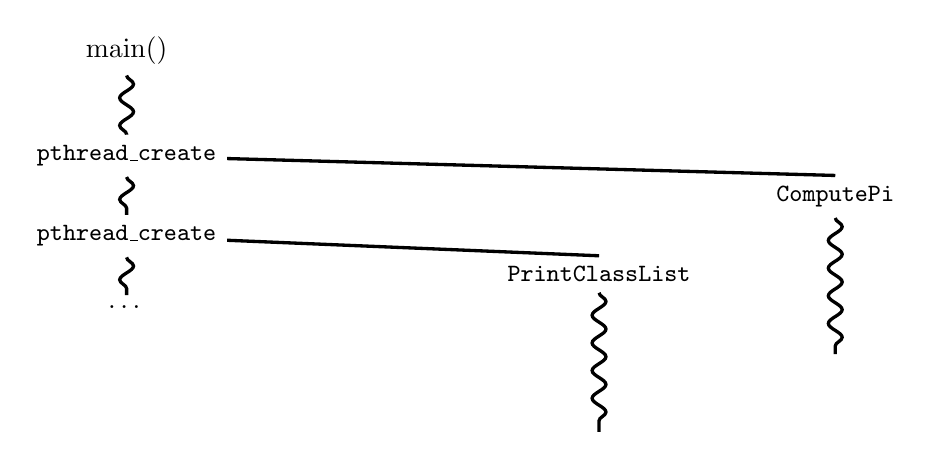
\begin{tikzpicture}
    \tikzset{
        thread/.style={very thick,draw,decorate,decoration=snake},
        split/.style={very thick,draw},
        marker/.style={thin,draw},
    }
    \draw[thread] (0, 0) node[above] {main()}-- ++(0, -.75) node[below,font=\tt\small] (create pi) {pthread\_create};
    \draw[thread] (create pi) -- ++(0, -.75) node[below,font=\tt\small] (create list) {pthread\_create};
    \draw[split] (create pi) -- ++(9, -.25) node[below,font=\tt\small] (computepi){ComputePi};
    \draw[thread] (computepi) -- ++(0, -2);
    \draw[thread] (create list) -- ++(0, -.75) node[below] {\ldots};
    \draw[split] (create list) -- ++(6, -.25) node[below,font=\tt\small] (classlist){PrintClassList};
    \draw[thread] (classlist) -- ++(0, -2);
\end{tikzpicture}
\end{frame}

\begin{frame}[fragile,label=pthreadCreateIntro]{pthread\_create}
\begin{lstlisting}[
    style=small,
    language=C++,
    moredelim={**[is][\btHL<2|handout:2>]{@2}{2@}},
    moredelim={**[is][\btHL<3|handout:3>]{@3}{3@}},
    moredelim={**[is][\btHL<4|handout:4>]{@4}{4@}},
    moredelim={**[is][\btHL<5|handout:5>]{@5}{5@}},
]
void *ComputePi(void *argument) { ...  }
void *PrintClassList(void *argument) { ...  }
int main() {
    pthread_t pi_thread, list_thread;
    pthread_create(&@2pi_thread2@, @4NULL4@, @3ComputePi3@, @4NULL4@);
    pthread_create(&@2list_thread2@, @4NULL4@, @3PrintClassList3@, @4NULL4@);
    ... /* more code */
}
\end{lstlisting}
    \begin{itemize}
    \item pthread\_create arguments:
    \item \myemph<2>{thread identifier}
    \item \myemph<3>{function to run}
        \begin{itemize}
        \item thread starts here, terminates if this function returns
        \end{itemize}
    \item \myemph<4>{thread attributes (extra settings) and function argument}
    \end{itemize}
\end{frame}




\subsection{exercise: pthread create race}
\usetikzlibrary{arrows.meta}
\begin{frame}<0>[fragile,label=pthreadCreateBrokenP]{a threading race}
\begin{lstlisting}[
    style=small,
    language=C++,
    moredelim={**[is][\btHL<1|handout:1>]{@1}{1@}},
]
#include <pthread.h>
#include <stdio.h>
void *print_message(void *ignored_argument) {
    @1printf("In the thread\n");1@ return NULL;
}
int main() {
    printf("About to start thread\n");
    pthread_t the_thread;
    pthread_create(&the_thread, NULL, print_message, NULL);
    printf("Done starting thread\n");
    return 0;
}
\end{lstlisting}
My machine: outputs \texttt{In the thread} \myemph{about 4\% of the time}. \\
What happened?
\end{frame}

\begin{frame}<0>[fragile,label=pthreadCreateRace]{a race}
\begin{itemize}
\item returning from main \myemph{exits the entire process} (all its threads)
    \begin{itemize}
    \item same as calling exit; not like other threads
    \end{itemize}
\item race: main's return 0 or print\_message's printf first?
\end{itemize}
\begin{tikzpicture}
\tikzset{
    box/.style={draw,thick},
    main box/.style={fill=blue!30},
    thread box/.style={fill=yellow!30},
    my label/.style={font=\small},
    >=Latex,
}
\draw[very thick,->] (0,1.25) -- (12,1.25) node[right] {time};
\path[main box] (0, 0) rectangle (8, 1) node[midway,my label]{main: printf/pthread\_create/printf/return};
\path[thread box] (5, -.5) rectangle (8, -1.5);
\path[thread box,fill=yellow!10,dashed] (8, -.5) rectangle (12, -1.5);
\path (5, -.5) rectangle (12, -1.5) node[midway,my label]{print\_message: printf/return};
\path[draw,thick,red] (8, 1) -- (8,-1.5) node[below,align=center] {return from main \\ ends all threads \\ in the process};
\end{tikzpicture}
\end{frame}



\begin{frame}[fragile,label=pthreadCreateBrokenP]{a threading race}
\begin{lstlisting}[
    style=small,
    language=C++,
    moredelim={**[is][\btHL<1|handout:1>]{@1}{1@}},
]
#include <pthread.h>
#include <stdio.h>
void *print_message(void *ignored_argument) {
    @1printf("In the thread\n");1@ return NULL;
}
int main() {
    printf("About to start thread\n");
    pthread_t the_thread;
    pthread_create(&the_thread, NULL, print_message, NULL);
    printf("Done starting thread\n");
    return 0;
}
\end{lstlisting}
My machine: outputs \texttt{In the thread} \myemph{about 4\% of the time}. \\
What happened?
\end{frame}

\begin{frame}[fragile,label=pthreadCreateRace]{a race}
\begin{itemize}
\item returning from main \myemph{exits the entire process} (all its threads)
    \begin{itemize}
    \item same as calling exit; not like other threads
    \end{itemize}
\item race: main's return 0 or print\_message's printf first?
\end{itemize}
\begin{tikzpicture}
\tikzset{
    box/.style={draw,thick},
    main box/.style={fill=blue!30},
    thread box/.style={fill=yellow!30},
    my label/.style={font=\small},
    >=Latex,
}
\draw[very thick,->] (0,1.25) -- (12,1.25) node[right] {time};
\path[main box] (0, 0) rectangle (8, 1) node[midway,my label]{main: printf/pthread\_create/printf/return};
\path[thread box] (5, -.5) rectangle (8, -1.5);
\path[thread box,fill=yellow!10,dashed] (8, -.5) rectangle (12, -1.5);
\path (5, -.5) rectangle (12, -1.5) node[midway,my label]{print\_message: printf/return};
\path[draw,thick,red] (8, 1) -- (8,-1.5) node[below,align=center] {return from main \\ ends all threads \\ in the process};
\end{tikzpicture}
\end{frame}

\begin{frame}[fragile,label=fixRace1]{fixing the race (version 1)}
\begin{lstlisting}[
    style=small,
    language=C++,
    moredelim={**[is][\btHL<1|handout:1>]{@1}{1@}},
]
#include <pthread.h>
#include <stdio.h>
void *print_message(void *ignored_argument) {
    printf("In the thread\n");
    return NULL;
}
int main() {
    printf("About to start thread\n");
    pthread_t the_thread;
    pthread_create(&the_thread, NULL, print_message, NULL);
    printf("Done starting thread\n");
    @1pthread_join(the_thread, NULL);1@  /* WAIT FOR THREAD */
    return 0;
}
\end{lstlisting}
\end{frame}

\begin{frame}[fragile,label=fixRace2]{fixing the race (version 2; not recommended)}
\begin{lstlisting}[
    style=small,
    language=C++,
    moredelim={**[is][\btHL<1|handout:1>]{@1}{1@}},
]
#include <pthread.h>
#include <stdio.h>
void *print_message(void *ignored_argument) {
    printf("In the thread\n");
    return NULL;
}
int main() {
    printf("About to start thread\n");
    pthread_t the_thread;
    pthread_create(&the_thread, NULL, print_message, NULL);
    printf("Done starting thread\n");
    @1pthread_exit(NULL);1@
}
\end{lstlisting}
\end{frame}



\subsection{pthread join and exit}


\begin{frame}{pthread\_join, pthread\_exit}
\begin{itemize}
\item \texttt{pthread\_join}: wait for thread, retrieves its return value
    \begin{itemize}
    \item like \texttt{waitpid}, but for a thread
    \item return value is pointer to anything
    \end{itemize}
\item \texttt{pthread\_exit}: exit current thread, returning a value
    \begin{itemize}
    \item like \texttt{exit} or returning from main, but for a single thread
    \item same effect as returning from function passed to pthread\_create
    \end{itemize}
\end{itemize}
\end{frame}


\subsection{on error checking}

\begin{frame}{a note on error checking}
\begin{itemize}
\item from pthread\_create manpage:
\end{itemize}
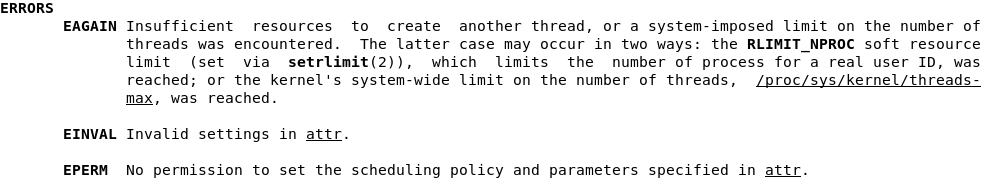
\includegraphics[width=\textwidth]{../threads/pthread-create-errors}
\begin{itemize}
\item special constants for \textit{return value}
\vspace{.5cm}
\item same pattern for many other pthreads functions
\item will often omit error checking in slides for brevity
\end{itemize}
\end{frame}

\begin{frame}[fragile,label=pthreadCreateErrorCheck]{error checking pthread\_create}
\begin{lstlisting}[language=C++,style=small]
int error = pthread_create(...);
if (error != 0) {
    /* print some error message */
}
\end{lstlisting}
\end{frame}


\subsection{parallel calculations in threads}

% FIXME: slide setting up the running example

\begin{frame}[fragile,label=sumToGlobal]{sum example (only globals)}
\begin{lstlisting}[
    language=C++,basicstyle=\tt\fontsize{9}{10}\selectfont,
    moredelim={**[is][\btHL<2|handout:2>]{@2}{2@}},
    moredelim={**[is][\btHL<3|handout:3>]{@3}{3@}},
    moredelim={**[is][\btHL<4|handout:4>]{@4}{4@}},
    escapeinside=QQ,
]
int @2values[1024]2@;  int @2results[2]2@;
void *sum_front(void *ignored_argument) {
    int sum = 0;
    for (int i = @303@; i < @35123@; ++i) { sum += values[i]; }
    @4results[@303@] = sum;4@
    return NULL;
}
void *sum_back(void *ignored_argument) {
    int sum = 0;
    for (int i = @35123@; i < @310243@; ++i) { sum += values[i]; }
    @4results[@313@] = sum;4@
    return NULL;
}
int sum_all() {
    pthread_t sum_front_thread, sum_back_thread;
    /* missing: error handling */
    pthread_create(&sum_front_thread, NULL, sum_front, NULL);
    pthread_create(&sum_back_thread, NULL, sum_back, NULL);
    pthread_join(sum_front_thread, NULL); pthread_join(sum_back_thread, NULL);
    return @4results[0] + results[1]4@;
}
\end{lstlisting}
\begin{tikzpicture}[overlay,remember picture]
\tikzset{
    box/.style={draw=red,very thick,fill=white,align=left}
}
    \begin{visibleenv}<2>
    \node[box,anchor=east] at ([yshift=-1.5cm,xshift=-1cm]current page.north east) {
        values, results: global variables --- shared
    };
    \end{visibleenv}
    \begin{visibleenv}<3>
    \node[box,anchor=east] at ([yshift=-1.5cm,xshift=-1cm]current page.north east) {
        two different functions \\
        happen to be the same except for some numbers
    };
    \end{visibleenv}
    \begin{visibleenv}<4>
    \node[box,anchor=east] at ([yshift=-1.5cm,xshift=-1cm]current page.north east) {
        values returned from threads \\
        via global array instead of return value \\
        (partly to illustrate that memory is shared, \\
        partly because this pattern works when we don't join (later))
    };
    \end{visibleenv}
\end{tikzpicture}
\end{frame}



\usetikzlibrary{calc,patterns,positioning}

\newcommand{\threadSumStackDecl}{
\tikzset{
    mylabel/.style={font=\ttfamily\fontsize{9}{10}\selectfont,black!70},
    mybox/.style={draw,rectangle,minimum width=5.5cm,fill=white},
    myhigh/.style={draw,rectangle,line width=1mm, draw=blue!80!black,opacity=.3},
    hilite stack/.style={draw=red,ultra thick},
}
}
\newcommand{\threadSumFirstStack}{thread two stack}
\newcommand{\threadSumSecondStack}{thread three stack}
\newcommand{\threadSumStackObjects}{
\node[mybox,minimum height=1cm,pattern=north west lines,pattern color=black!5!white] (kernel) {Used by OS};
\begin{pgfonlayer}{bg}
\node[right=1mm of kernel.north east,mylabel] (topLabel) {0xFFFF FFFF FFFF FFFF};
\node[right=1mm of kernel.south east,mylabel] {0xFFFF 8000 0000 0000};
\end{pgfonlayer}
\node[mybox, minimum height=.5cm, below=1cm of kernel] (stack 1) {main thread stack};
\begin{pgfonlayer}{bg}
\node[right=1mm of stack 1.north east,mylabel] {0x7F\ldots{}};
\end{pgfonlayer}
\node[mybox, minimum height=.5cm, below=0.5cm of stack 1] (stack 2) {\threadSumFirstStack};
\node[mybox, minimum height=.5cm, below=0.25cm of stack 2] (stack 3) {\threadSumSecondStack};
\node[mybox, minimum height=.5cm, below=0.25cm of stack 3] (heap) {Heap / other dynamic};
\node[mybox, minimum height=.5cm, below=0mm of heap] (sdata) {Code / Data};
\begin{pgfonlayer}{bg}
\node[yshift=-1mm,right=1mm of sdata.south east,mylabel] (bottomLabel) {0x0000 0000 0040 0000};
\end{pgfonlayer}
\coordinate (memBottom) at ($(sdata.south east) + (0mm, -2mm)$);
\begin{pgfonlayer}{bg}
\draw[pattern=north west lines, pattern color=black!40!white] (kernel.north west) rectangle (memBottom);
\end{pgfonlayer}
}

\usetikzlibrary{matrix}

\begin{frame}[fragile,label=threadSumMemoryGlobals]{thread\_sum memory layout}
\begin{tikzpicture}
\threadSumStackDecl
\renewcommand{\threadSumFirstStack}{\small \texttt{sum\_front\_thread} stack}
\renewcommand{\threadSumSecondStack}{\small \texttt{sum\_back\_thread} stack}
\threadSumStackObjects
\draw[very thick,blue] ([yshift=2mm]sdata.west) rectangle ([yshift=3mm]sdata.east);
\node[anchor=west,blue!70!black] (sdata arr) at ([xshift=-1mm,yshift=4mm]sdata.east) { values, results (global) };
\begin{visibleenv}<2->
\matrix[draw,anchor=north east,tight matrix,nodes={font=\fontsize{9}{10}\selectfont,text width=2cm},
    label={[font=\fontsize{9}{10}\selectfont]north:sum\_front thread}] at
    ([xshift=8cm,yshift=4cm]sdata.east)
{
|[alias=front pc]| PC \\
|[alias=front regs]| registers \\
\ldots \\
};
\matrix[draw,anchor=north east,tight matrix,nodes={font=\fontsize{9}{10}\selectfont,text width=2cm},
    label={[font=\fontsize{9}{10}\selectfont]north:sum\_back thread}] at
    ([xshift=8cm,yshift=2cm]sdata.east)
{
|[alias=back pc]| PC \\
|[alias=back regs]| registers \\
\ldots \\
};
\draw[green!70!black,thick,<-] ([yshift=-2mm]sdata.east) -- ++(1, 0) node[right,yshift=-1mm,fill=white,font=\fontsize{10}{11}\selectfont,inner sep=0.1mm] {
        sum\_front
} -- ++(8, 0) |- ([xshift=-1cm]front pc.east);
\draw[green!70!black,thick,<-] ([yshift=0mm]sdata.east) -- ++(5, 0) node[right,fill=white,font=\fontsize{10}{11}\selectfont,inner sep=0.1mm,yshift=1mm] {
        sum\_back
} -- ++(3.25, 0) |- ([xshift=-1cm]back pc.east);
\draw[green!70!black,->] ([xshift=.5mm,yshift=1mm]front regs.west) -- ++(-3, 0) |- (stack 2.east);
\draw[green!70!black,->] ([xshift=.5mm,yshift=1mm]back regs.west) -- ++(-3, 0) |- (stack 3.east);
\end{visibleenv}
\end{tikzpicture}
\end{frame}



\subsection{passing info to threads}

\subsubsection{thread ID as argument}
% FIXME: show thread registers?

\begin{frame}[fragile,label=sumToGlobalWithId]{sum example (to global, with thread IDs)}
\begin{lstlisting}[
    language=C++,basicstyle=\tt\fontsize{9}{10}\selectfont,
    moredelim={**[is][\btHL<2|handout:2>]{@2}{2@}},
    moredelim={**[is][\btHL<3|handout:3>]{@3}{3@}},
    moredelim={**[is][\btHL<4|handout:4>]{@4}{4@}},
    escapeinside=QQ,
]
int @2values[1024]2@;
int @2results[2]2@;
void *sum_thread(void *argument) {
    int id = (int) argument;
    int sum = 0;
    for (int i = id * 512; i < (id + 1) * 512; ++i) {
        sum += values[i];
    }
    results[id] = sum;
    return NULL;
}
int sum_all() {
    /* missing: error handling */
    pthread_t thread[2];
    for (int i = 0; i < 2; ++i) {
        pthread_create(&threads[i], NULL, sum_thread, (void *) i);
    }
    for (int i = 0; i < 2; ++i)
        pthread_join(threads[i], NULL);
    return results[0] + results[1];
}
\end{lstlisting}
\begin{tikzpicture}[overlay,remember picture]
\tikzset{
    box/.style={draw=red,very thick,fill=white,align=left}
}
    \begin{visibleenv}<2>
    \node[box,anchor=east] at ([yshift=-2cm,xshift=-1cm]current page.north east) {
        values, results: global variables --- shared
    };
    \end{visibleenv}
\end{tikzpicture}
\end{frame}


\subsubsection{globals + info struct as argument}
\begin{frame}[fragile,label=sumToStack]{sum example (info struct)}
\begin{lstlisting}[
    language=C++,basicstyle=\tt\fontsize{9}{10}\selectfont,
    moredelim={**[is][\btHL<2|handout:2>]{@2}{2@}},
    moredelim={**[is][\btHL<3|handout:3>]{@3}{3@}},
    moredelim={**[is][\btHL<4|handout:4>]{@4}{4@}},
    escapeinside=QQ,
]
int @2values[1024];2@ Q\tikzmark{array}Q
struct ThreadInfo {
    int start, end, result;
};
void *sum_thread(void *argument) {
    ThreadInfo *@3my_info3@ = Q\tikzmark{info}Q (ThreadInfo *) argument;
    int sum = 0;
    for (int i = my_info->start; i < my_info->end; ++i) { sum += values[i]; }
    @4my_info->result = sum;4@
    return NULL;
}
int sum_all() {
    pthread_t thread[2]; @3ThreadInfo info[2];3@
    for (int i = 0; i < 2; ++i) {
        info[i].start = i*512; info[i].end = (i+1)*512;
        pthread_create(&threads[i], NULL, sum_thread, &info[i]);
    }
    for (int i = 0; i < 2; ++i) { pthread_join(threads[i], NULL); }
    return info[0].result + info[1].result;
}
\end{lstlisting}
\begin{tikzpicture}[overlay,remember picture]
\tikzset{
    box/.style={draw=red,very thick,fill=white,align=left}
}
    \begin{visibleenv}<2>
    \node[box,anchor=west] at (pic cs:array) {
        values: global variable --- shared
    };
    \end{visibleenv}
    \begin{visibleenv}<3>
    \node[box,anchor=north west] at (pic cs:info) {
        my\_info: pointer to sum\_all's stack \\
        only okay because sum\_all waits!
    };
    \end{visibleenv}
\end{tikzpicture}
\end{frame}

\usetikzlibrary{arrows.meta}

\begin{frame}[fragile,label=threadSumMemoryGlobalAndStacks]{thread\_sum memory layout (info struct)}
\begin{tikzpicture}
\threadSumStackDecl
\renewcommand{\threadSumFirstStack}{\small \texttt{threads[0]} stack}
\renewcommand{\threadSumSecondStack}{\small \texttt{threads[1]} stack}
\threadSumStackObjects
    \draw[very thick,blue] ([yshift=2mm]sdata.west) rectangle ([yshift=3mm]sdata.east);
    \node[anchor=west,blue!70!black] (sdata arr) at ([xshift=0cm,yshift=2.5mm]sdata.east) { values (global) };

    \node[anchor=west,blue!70!black] (info arr) at ([xshift=.5cm]stack 1.east) { info array };
    \draw[very thick,blue] ([yshift=-0mm]stack 1.west) rectangle ([yshift=-1mm]stack 1.east);

    \node[anchor=west] (my info ptr) at ([xshift=0cm]stack 2.east) { my\_info };
    \draw[-Latex] (my info ptr.east) -- ++ (1cm, 0cm) |- ([yshift=-1mm]info arr.east);
    \node[anchor=west] (my info ptr 2) at ([xshift=0cm]stack 3.east) { my\_info };
    \draw[-Latex] (my info ptr 2.east) -- ++ (1.1cm, 0cm) |- ([yshift=1mm]info arr.east);
\end{tikzpicture}
\end{frame}




\subsubsection{no globals + info struct as argument}
\begin{frame}[fragile,label=sumNoGlobals]{sum example (to main stack)}
\begin{lstlisting}[
    language=C++,basicstyle=\tt\fontsize{9}{10}\selectfont,
    moredelim={**[is][\btHL<2|handout:2>]{@2}{2@}},
    moredelim={**[is][\btHL<3|handout:3>]{@3}{3@}},
    moredelim={**[is][\btHL<4|handout:4>]{@4}{4@}},
    escapeinside=QQ,
]
struct ThreadInfo { @2int *values;2@ int start; int end; int result };
void *sum_thread(void *argument) {
    ThreadInfo *@3my_info3@ = (ThreadInfo *) argument;Q\tikzmark{info}Q
    int sum = 0;
    for (int i = my_info->start; i < my_info->end; ++i) {
        sum += my_info->values[i];
    }
    @4my_info->result = sum;4@
    return NULL;

}
int sum_all(int *values) {
    ThreadInfo info[2]; pthread_t thread[2];
    for (int i = 0; i < 2; ++i) {
        @2info[i].values = values;2@ info[i].start = i*512; info[i].end = (i+1)*512;
        pthread_create(&threads[i], NULL, sum_thread, (void *) &info[i]);
    }
    for (int i = 0; i < 2; ++i)
        pthread_join(threads[i], NULL);
    return info[0].result + info[1].result;
}
\end{lstlisting}
\end{frame}

\usetikzlibrary{arrows.meta}
\begin{frame}{program memory (to main stack)}
\begin{tikzpicture}
\threadSumStackDecl
\renewcommand{\threadSumFirstStack}{\small first thread stack}
\renewcommand{\threadSumSecondStack}{\small second thread stack}
\threadSumStackObjects

    \node[anchor=west,blue!70!black] (info arr) at ([xshift=.5cm]stack 1.east) { info array };
    \draw[very thick,blue] ([yshift=-0mm]stack 1.west) rectangle ([yshift=1mm]stack 1.east);
    \draw[-Latex] ([yshift=1.5mm]info arr.east) -- ++(2cm,0cm) node[right,yshift=0mm] { values (stack? heap?)};
    \draw[-Latex] ([yshift=-0.5mm]info arr.east) -- ++(2cm,0cm);
    
    \node[anchor=west,font=\it] (my info ptr) at ([xshift=0cm]stack 2.east) { my\_info };
    \draw[-Latex] (my info ptr.east) -- ++ (1cm, 0cm) |- ([yshift=-1mm]info arr.east);

    \node[anchor=west,font=\it] (my info ptr 2) at ([xshift=0cm]stack 3.east) { my\_info };
    \draw[-Latex] (my info ptr 2.east) -- ++ (1.25cm, 0cm) |- ([yshift=1mm]info arr.east);
\end{tikzpicture}
\end{frame}


\subsubsection{everything on the heap}
\begin{frame}[fragile,label=sumAllHeap]{sum example (on heap)}
\begin{lstlisting}[
    language=C++,basicstyle=\tt\fontsize{9}{10}\selectfont,
    moredelim={**[is][\btHL<2|handout:2>]{@2}{2@}},
    moredelim={**[is][\btHL<3|handout:3>]{@3}{3@}},
    moredelim={**[is][\btHL<4|handout:4>]{@4}{4@}},
    escapeinside=QQ,
]
struct ThreadInfo { @3pthread_t thread;3@ int *values; int start; int end; int result };
void *sum_thread(void *argument) {
    ...
}

struct ThreadInfo *start_sum_all(int *values) {
    struct ThreadInfo *info = @2calloc(2, sizeof(struct ThreadInfo);2@
    for (int i = 0; i < 2; ++i) {
        info[i].values = values; info[i].start = i*512; info[i].end = (i+1)*512;
        pthread_create(&info[i].thread, NULL, sum_thread, (void *) @2&info[i]2@);
    }
    return info;
}

int finish_sum_all(ThreadInfo *info) {
    for (int i = 0; i < 2; ++i)
        pthread_join(@3info[i].thread3@, NULL);
    int result = info[0].result + info[1].result;
    free(info);
    return result;
}
\end{lstlisting}
\end{frame}


\usetikzlibrary{arrows.meta}
\begin{frame}[fragile,label=threadSumMemoryHeap]{thread\_sum memory (heap version)}
\begin{tikzpicture}
\threadSumStackDecl
    \renewcommand{\threadSumFirstStack}{\small first thread stack}
    \renewcommand{\threadSumSecondStack}{\small second thread stack}
\threadSumStackObjects
    \node[anchor=west,blue!70!black] (info arr) at ([xshift=.5cm]heap.east) { info array };
    \draw[very thick,blue] ([yshift=-0mm]heap.west) rectangle ([yshift=1mm]heap.east);
    \draw[-Latex] ([yshift=1.5mm]info arr.east) -- ++(2cm,0cm) node[right,yshift=-1mm] { values (stack? heap?)};
    \draw[-Latex] ([yshift=-0.5mm]info arr.east) -- ++(2cm,0cm);
    \node[anchor=west,font=\it] (my info ptr 2) at ([xshift=0cm]stack 3.east) { my\_info };
    \draw[-Latex] (my info ptr 2.east) -- ++ (1.25cm, 0cm) |- ([yshift=-1mm]info arr.east);
    \node[anchor=west,font=\it] (my info ptr) at ([xshift=0cm]stack 2.east) { my\_info };
    \draw[-Latex] (my info ptr.east) -- ++ (1.5cm, 0cm) |- ([yshift=1mm]info arr.east);
\end{tikzpicture}
\end{frame}


\subsection{on thread resources, detached threads}

\subsubsection{exercise}

\usetikzlibrary{calc,decorations.pathreplacing,patterns,positioning}
\begin{frame}[fragile,label=stackLeak]{what's wrong with this?}
\begin{lstlisting}[language=C++,style=small]
/* omitted: headers */
void *create_string(void *ignored_argument) {
  char string[1024];
  ComputeString(string);
  return string;
}
int main() {
  pthread_t the_thread;
  pthread_create(&the_thread, NULL, create_string, NULL);
  char *string_ptr;
  pthread_join(the_thread, (void**) &string_ptr);
  printf("string is %s\n", string_ptr);
}
\end{lstlisting}
\end{frame}

\begin{frame}{program memory}
\begin{tikzpicture}
\tikzset{
    mylabel/.style={font=\ttfamily},
    mybox/.style={draw,rectangle,minimum width=5cm,fill=white},
    myhigh/.style={draw,rectangle,line width=1mm, draw=blue!80!black,opacity=.3},
    hilite stack/.style={draw=red,ultra thick},
}
\node[mybox,minimum height=1cm,pattern=north west lines,pattern color=black!5!white] (kernel) {Used by OS};
\begin{pgfonlayer}{bg}
\node[right=1mm of kernel.north east,mylabel] (topLabel) {0xFFFF FFFF FFFF FFFF};
\node[right=1mm of kernel.south east,mylabel] {0xFFFF 8000 0000 0000};
\end{pgfonlayer}
\node[mybox, minimum height=.5cm, below=1cm of kernel] (stack 1) {main thread stack};
\begin{pgfonlayer}{bg}
\node[right=1mm of stack 1.north east,mylabel] {0x7F\ldots{}};
\end{pgfonlayer}
\node[mybox, minimum height=.5cm, below=0.5cm of stack 1,hilite stack,alt=<2>{opacity=0.5}] (stack 2) {second thread stack};
\node[mybox, minimum height=.5cm, below=0.25cm of stack 2,hilite stack,alt=<2>{opacity=0.5}] (stack 3) {third thread stack};
\node[mybox, minimum height=.5cm, below=0.25cm of stack 3] (heap) {Heap / other dynamic};
\node[mybox, minimum height=.5cm, below=0mm of heap] (sdata) {Code / Data};
\begin{pgfonlayer}{bg}
\node[right=1mm of sdata.south east,mylabel] (bottomLabel) {0x0000 0000 0040 0000};
\end{pgfonlayer}
\coordinate (memBottom) at ($(sdata.south east) + (0mm, -2mm)$);
\begin{pgfonlayer}{bg}
\draw[pattern=north west lines, pattern color=black!40!white] (kernel.north west) rectangle (memBottom);
\end{pgfonlayer}
\draw[decorate,decoration={brace},red,ultra thick] ([xshift=.25cm]stack 2.north east) -- ([xshift=.25cm]stack 3.south east) node[midway,right,align=left](dynamicStackBox) {
    dynamically allocated stacks \\
    \texttt{char string[]} allocated here  \\
    \texttt{string\_ptr} pointed to here
};
\node[anchor=north,align=left] at ([yshift=-1cm]dynamicStackBox) {
    \ldots stacks deallocated when \\ threads exit/are joined
};
\end{tikzpicture}
\end{frame}




\subsubsection{join, detach, etc.}
\begin{frame}{thread resources}
\begin{itemize}
\item to create a thread, allocate:
\item new stack (how big???)
\item thread control block
\vspace{.5cm}
\item deallocated when \ldots
\item<2-> can deallocate stack when thread exits
\item<2-> but need to allow collecting return value
    \begin{itemize}
    \item same problem as for processes and waitpid
    \end{itemize}
\end{itemize}
\end{frame}

\begin{frame}[fragile,label=pthreadDetach]{pthread\_detach}
\begin{lstlisting}[
    style=smaller,
    language=C++,
    moredelim={**[is][\btHL<1|handout:1>]{@1}{1@}},
]
void *show_progress(void * ...) { ... }
void spawn_show_progress_thread() {
    pthread_t show_progress_thread;
    pthread_create(&show_progress_thread, NULL,
                   show_progress, NULL);

    /* instead of keeping pthread_t around to join thread later: */
    @1pthread_detach(show_progress_thread);1@
}

int main() {
    spawn_show_progress_thread();
    do_other_stuff();
    ...
}
\end{lstlisting}
\begin{tikzpicture}[overlay,remember picture]
\coordinate (place) at ([yshift=1cm]current page.south);
\node[align=left,draw=red,ultra thick,anchor=south,at={(place)}] {
    detach = don't care about return value, etc.\\
    system will deallocate when thread terminates
};
\end{tikzpicture}
\end{frame}

\begin{frame}[fragile,label=startThreadDetached]{starting threads detached}
\begin{lstlisting}[
    style=smaller,
    language=C++,
    moredelim={**[is][\btHL<1|handout:1>]{@1}{1@}},
]
void *show_progress(void * ...) { ... }
void spawn_show_progress_thread() {
    pthread_t show_progress_thread;
    pthread_attr_t attrs;
    pthread_attr_init(&attrs);
    @1pthread_attr_setdetachstate(&attrs, PTHREAD_CREATE_DETACHED);1@
    pthread_create(&show_progress_thread, attrs,
                   show_progress, NULL);
    pthread_attr_destroy(&attrs);
}
\end{lstlisting}
\end{frame}

\begin{frame}[fragile,label=setStackSize]{setting stack sizes}
\begin{lstlisting}[
    style=small,
    language=C++,
    moredelim={**[is][\btHL<1|handout:1>]{@1}{1@}},
]
void *show_progress(void * ...) { ... }
void spawn_show_progress_thread() {
    pthread_t show_progress_thread;
    pthread_attr_t attrs;
    pthread_attr_init(&attrs);
    @1pthread_attr_setstacksize(&attrs, 32 * 1024 /* bytes */);1@
    pthread_create(&show_progress_thread, attrs,
                   show_progress, NULL);
}
\end{lstlisting}
\end{frame}






\section{backup slides}
\begin{frame}{backup slides}
\end{frame}

\end{document}
